%===========================================================
% 3. Brent法
%===========================================================
\section{黄金分割法と放物線補間の融合}

\begin{frame}
 \frametitle{Brent法のコンセプト}
 
 \textbf{基本的な考え方:}
  各反復で「どちらの戦略を使うか」を判定
  \begin{itemize}
   \item 放物線補間が信頼できそう $\Rightarrow$ 使う
   \item そうでない $\Rightarrow$ 黄金分割に切り替え
 \end{itemize}
\end{frame}
\begin{frame}
  常に3つの良い候補点 $(x, w, v)$ と 極値が必ず存在する区間 $[a^*, b^*]$ を保持
  \begin{itemize}
   \item $x$：現在の最良点（最も良い関数値）
   \item $w$：2番目に良い点
   \item $v$：3番目に良い点（または直前の$w$）
   \item $a^*$：極値が存在する区間の左端点 
   \item $b^*$：極値が存在する区間の右端点
  \end{itemize}
  
  条件によって二つの手法を取る
  \begin{itemize}
   \item  $x,w,v$ を用いて放物線補間で次の点を探す
   \item  $a^*,x ,b^*$ と黄金分割で堅実さを保証
  \end{itemize}
\end{frame}

\begin{frame}
 \frametitle{Brent法：強制二分条件}

 \textbf{放物線補間を採用するための判断条件:}
 前々回の$x$から試みた移動距離 $e$、今回の放物線補間による軸と現在の$x$との距離を $d$ とするとき、
 以下を満たさなければならない：
 
 \begin{tcolorbox}[colback=red!10!white, colframe=red!75!black, title=強制二分条件]
  \begin{equation*}
   |d| < \frac{1}{2}|e|
  \end{equation*}
 \end{tcolorbox}
\end{frame}

%% Brent法の収束過程のグラフをここに貼る

% Brent法のアニメーション
\begin{frame}{Brent法：ハイブリッド戦略の可視化}
  \begin{columns}
    \begin{column}{0.4\textwidth}
      \begin{itemize}
        \item \textbf{グレー領域}: 解を囲む区間 $[a, b]$
        \item \textcolor{blue}{\textbf{青丸}}: 現在の主要な3点 ($x, w, v$)
        \item \textcolor{red}{\textbf{赤丸}}: 今回の試行点 $u$
        \item \textcolor{green}{\textbf{緑破線}}: 採用された近似放物線
      \end{itemize}
      \vspace{1em}
      \small
      基本は放物線補間を試み、条件が悪い場合（緑線が出ない回）は安全な黄金分割を選択している様子がわかる。
    \end{column}
    \begin{column}{0.6\textwidth}
      \centering
      \only<1>{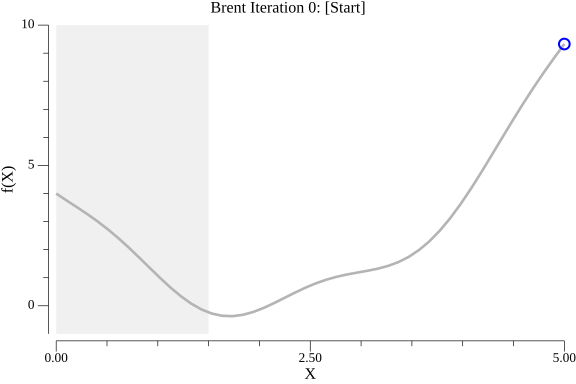
\includegraphics[width=\textwidth]{material/brent/output/brent_00.png}}
      \only<2>{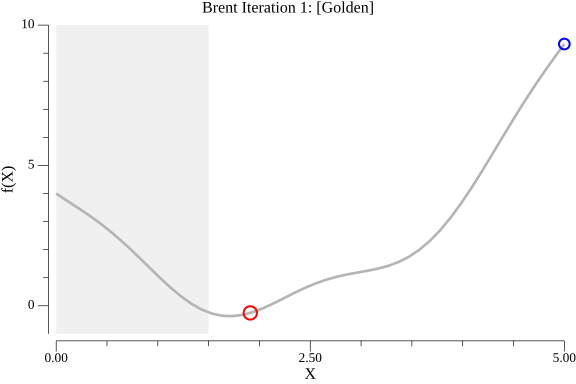
\includegraphics[width=\textwidth]{material/brent/output/brent_01.png}}
      \only<3>{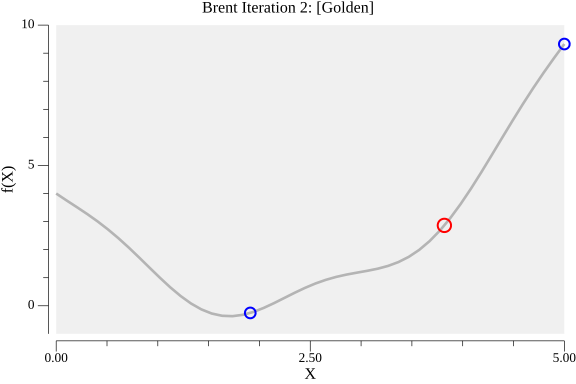
\includegraphics[width=\textwidth]{material/brent/output/brent_02.png}}
      \only<4>{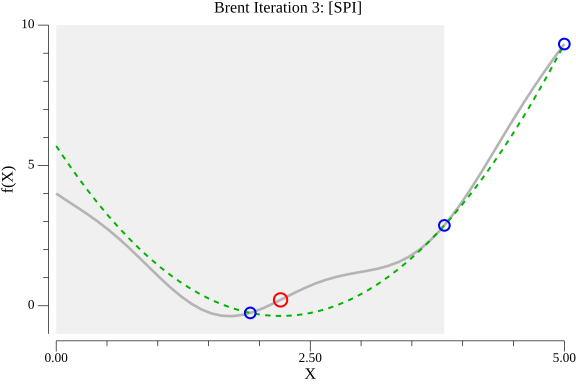
\includegraphics[width=\textwidth]{material/brent/output/brent_03.png}}
      \only<5>{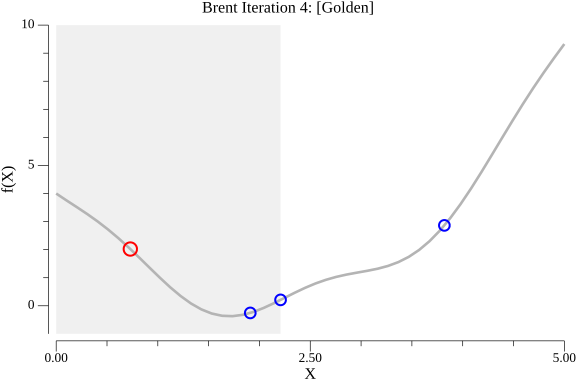
\includegraphics[width=\textwidth]{material/brent/output/brent_04.png}}
      \only<6>{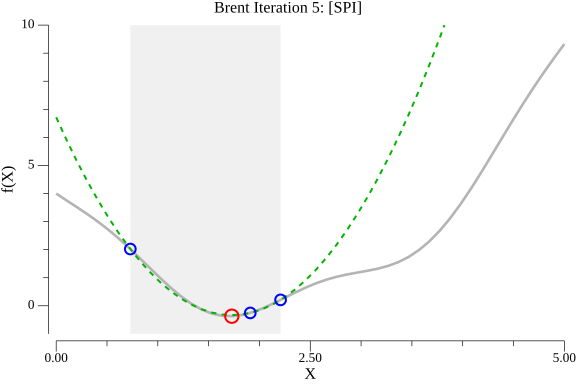
\includegraphics[width=\textwidth]{material/brent/output/brent_05.png}}
      \only<7>{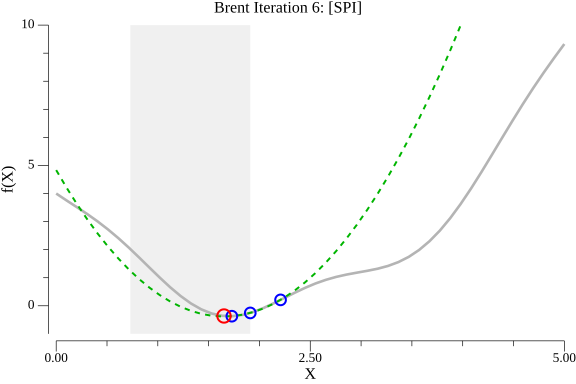
\includegraphics[width=\textwidth]{material/brent/output/brent_06.png}}
      \only<8>{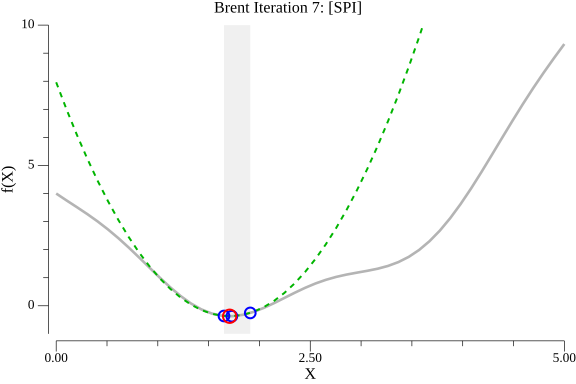
\includegraphics[width=\textwidth]{material/brent/output/brent_07.png}}
      \only<9>{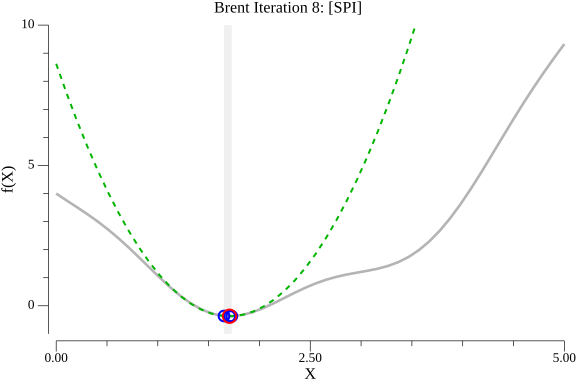
\includegraphics[width=\textwidth]{material/brent/output/brent_08.png}}
      \only<10>{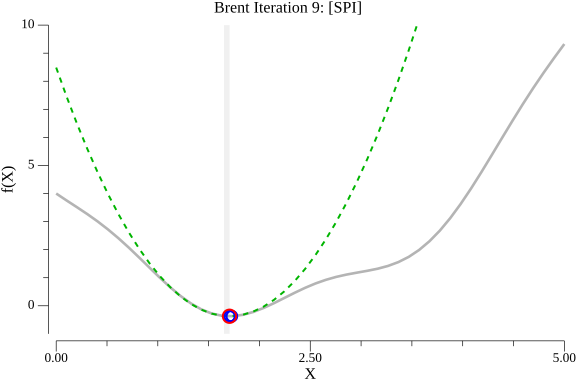
\includegraphics[width=\textwidth]{material/brent/output/brent_09.png}}
      \only<11>{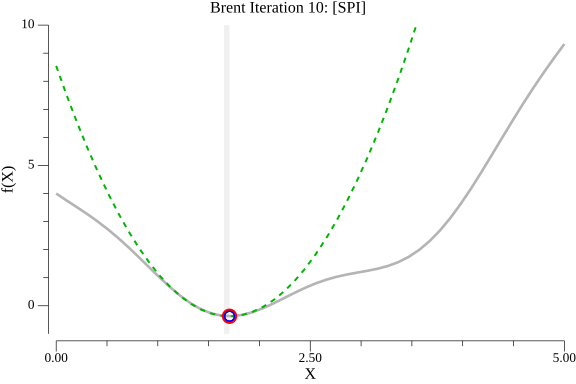
\includegraphics[width=\textwidth]{material/brent/output/brent_10.png}}
      \only<12>{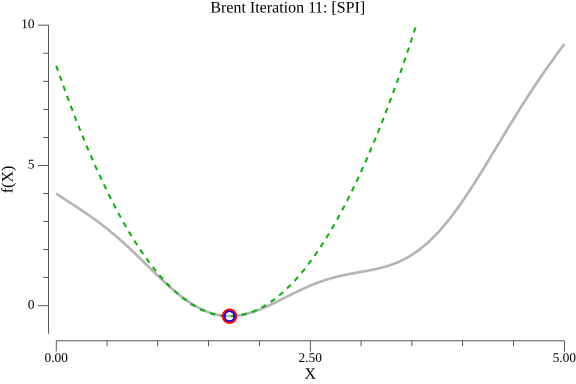
\includegraphics[width=\textwidth]{material/brent/output/brent_11.png}}
      \only<13>{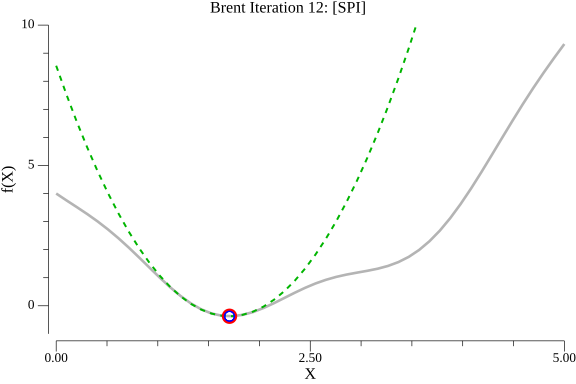
\includegraphics[width=\textwidth]{material/brent/output/brent_12.png}}
    \end{column}
  \end{columns}
\end{frame}
